\section{Introduction a la visualisation de données}

La visualisation représente l'étape d'observation du cycle \textit{Observation -> Théorie -> Expérience} puisque c'est cette étape qui boucle la boucle.
La visualisation représente la premiere étape dans l'observation de la simulation.
Elle a pour but d'être une première approche qualitative qui va ensuite permettre de cibler une seconde approche plus quantitative.
Par exemple, on peux utiliser une visualisation des la distribution du gaz dans certaine galaxie pour identifier la forme des galaxies, pour ensuite chercher a quantifier leurs forme en fonction de leurs halo hote.
On peut facilement observer a l'oeil les motifs en forme de papillon des bulles d'ionisation.
Ou la structure en réseau de la matière a grande échelle.

Le cerveaux humain est efficace pour identifier les pattern visuels. 
La visualisation de donnée scientifique est importante car elle permet d'obtenir énormément d'information.



%pour qui?
Il existe tout un panel de visualisation possible, et avant même de définir un but il faut définir une cible car les outils ne seront pas les mêmes en fonction de la cible a laquelle ils s'adressent.
On distinguera principalement trois catégories de public:

\begin{itemize}
\item Le grand public.
\item L'éducation.
\item Les professionnels.
\end{itemize}

Le grand public sera touché par les images de vulgarisations que l'on peut trouver sur internet ou dans les magasine.
Ce type d'image n'a pour seul but que d'être artistique et agréable a regarder.

Les images a vocation éducatives se doivent aussi d'être belles, mais elles doivent également comporter une partie informatives.
Elle doivent contenir une certaine dose d'information supplémentaire par rapport aux images purement artistique.

Enfin les outils de visualisation pour les professionnel disposes généralement de tous les outils nécessaire a la quantification de l'information.
On pourra par exemple analyser différents champs physique, sous différents angles, on pourra changer les échelles de couleurs, etc.

% L'éducation 
%Ratio équitable entre qualification et quantification

%/ La vulgarisation
%Qualification principalement 
%il est important de créer des belles image

%Aligner des 1 et des 0 sur des gros ordinateur, n'a vraiment de sens que si il représente quelque chose.
%Le mot important dans cette phrase est représentation.
%Il est nécessaire, en recherche de visualiser ce qui se passe dans les simulations pour comprendre et qualifier les phénomènes avant de pouvoir les quantifier.
%Cette cible aura besoin d'outils pointu aillant pour principal objectif la quantification.

Le principal défi de la visualisation des simulation cosmologique est la quantité de données qu'elles représente.
Si il est possible de faire des rendu pré-calculés d'images, il est encore impossible d'avoir une représentation en temps réel.
Pourtant il existe des techniques (dans le monde des jeux vidéo par exemple) permettant d'afficher dynamiquement des univers en 3 dimensions gigantesque de manière fluide sur des machines grand public.
Je pense qu'il y a de quoi s'inspirer de ce coté la.

%Pourquoi

%Le monde de la 3D.
%Les simus, les moteurs de jeux video, les SFX de films,
%La 3D est partout.
%Les monde des simulation peux s'en inspirer.


\section{Projeter une grille AMR}

Pour rappel, le format de donnée en sortie d'EMMA, sont sous forme de liste de cellules AMR dans un  espace en 3 dimensions..
Une image (en nuance de gris) est composée d'une matrice a 2 dimensions de pixel réguliers en forme et en taille.
Il est donc necéssaire d'effectuer une transformation entre ces deux représentation.
Comme cette transformation mène a la perte d'une dimension on parlera de projection.

\subsection{Le tirage des lignes de visées}

La représentation d'un environnement virtuel a 3 dimensions passe toujours par la création d'une image a deux dimensions.
Il existe différents types de méthodes de projections qui dépendent de la gestion des lignes de visées.
Dans la suite de ce chapitre nous allons développer deux d'entre elles: la projection en perspective et la projection orthogonale (Fig \ref{fig:raycast_projection}).

\paragraph{La projection orthogonale} correspond a l'approximation de grande distance.
Les rayons sont parallèles entre eux et le cube de données est comme "écrasée" ou "imprimée" suivant un axe.
Cette projection est moins naturelle, dans le sens ou elle ne correspond pas a ce que nous avons l'habitude de percevoir, mais elle a l'avantage d'être relativement simple a mettre en œuvre.

\paragraph{La projection en perspective} correspond au cas l'observateur est ponctuel et au centre d'une sphere, les rayons lumineux lui arrive radialement.
C'est la projection qui se rapproche le plus de la vision "naturelle".

\begin{figure}[bth]
    \center
    \subfloat[Orthogonale]{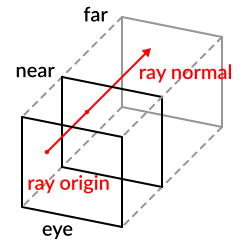
\includegraphics[width=0.45\textwidth]{img/04/raycast_ortho.png}}%
    \qquad
   	\subfloat[Perspective]{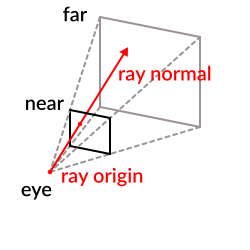
\includegraphics[width=0.45\textwidth]{img/04/raycast_perspective.png}}%
    \caption{Les deux types de projections que nous allons aborder.}
 	\label{fig:raycast_projection}
\end{figure}


\subsection{La réduction des lignes de visées}

Une fois les lignes de visées obtenues, il faut les réduire une valeur unique pour effectuer la projection
Il existe plusieurs (une infinité de) façons de réduire les lignes de visées, en voici quelques une que j'ai pu utiliser:

\begin{itemize}
\item La moyenne ou la somme ont l'avantage d'être facilement implémentable et de garder l'information sur toute la ligne de visée.

\item Le maximum permet d'augmenter significativement le contraste, rendant les images visuellement plus intéressante que la somme mais en contre partie certaines projections peuvent présenter des artefacts indésirables.

\item L'épaisseur optique permet de garder de l'information sur toute la ligne et d'être une représentation avec une signification physique car elle utilise les équations de transfert du rayonnement.
Cependant elle est plus gourmande en ressources.
Pour faire de la visualisation pure on pourra utiliser une expression du type:
\begin{equation}
v= \sum e^{-x}
\end{equation}
Et on pourra également être plus quantitatif en utilisant les vraies équations physique mais il faudra utiliser plusieurs champs simultanément. %TODO ref
\end{itemize}

%Une des méthodes les plus facile consiste a prendre la moyenne ou la somme de la ligne, cette méthode présente l'avantage de représenter l'ensemble de la ligne.
%Il est également possible de prendre les maximum de la ligne, cette méthode augmente significativement le contraste, au point que certaines projections peuvent présenter des artefacts indésirables.

%Une troisième méthodes légèrement plus physique consiste a utiliser les équations de transfert du rayonnment pour determiner l'epaisseur optique de la ligne

%Enfin, il est possible d'utilisé la réelle expression de l'epaisseur optique, prenant en compte densité, température, ionization et vitesse du gaz.
%(TODO)

\section{Projection orthogonale}

J'ai développer une méthode de projection d'AMR sur une grille (2D ou 3D) de taille arbitraire en utilisant les fonctions histogramme de Numpy.
Ces fonctions étant binen optimisées, la performance de génération de cube est généralement satisfaisante (de l'ordre de quelque secondes pour un cube de $1024^3$).
L'idée est de considéré les cellule AMR comme des particules d'une certaine taille.

Prenons l'exemple d'une grille de densité non raffiné utilisant les sorties EMMA.
Une grille 2D quelconque est représenté par le couple $x,y$ étant les positions du bord inférieur gauche des cellules, $l$ étant le niveau des cellules et $d$  étant le champs a représenter (prenons par exemple la densité).

Le volume de la cellule est définis en fonction du niveau suivant:
\begin{equation}
dV= 2^{-3L}
\end{equation} 


En réalisant un histogram 2d de x et y pondéré en masse.
Le poids de chaque cellule correspond a la masse de la cellule $w = \rho \cdot dV$:
En considérant le centre des cellule $(x' = x+dx(L) /2)$ et en ajustant le bin de l'histograme sur la taille de la grille on peux projeter un niveau rapidement.

%\begin{lstlisting}[float=bth,language=python,frame=tb,caption={lprojection de l'AMR par la méthode des histogramme Numpy},label=lst:useless]
% import numpy as np
% h,binX,binY=np.hystogram2d(x,y,weight=dv)
%\end{lstlisting}
o%u h est une matrice 2d representant la projection.


Lorsque l'AMR d'entrée contient plusieurs niveaux, il est possible de projeter les cellules niveau par niveau.
Par example pour une grille contenant les niveaux 8 et 9, on projettera d'abord toutes les cellules de niveau 8 pour obtenir une matrice $256x256$.
On agrandira cette matrice avec des opérateurs de changement de grille (cf Section \ref{Opérateurs de changement de grilles}).
%La méthode la plus naturelle consiste utiliser une projection directe.
Nous obtenons alors une première grille de taille $512x512$.
On projettera ensuite  de la même manière les cellules du niveau $9$ pour obtenir une seconde matrice de taille $512x512$.
En prenant la moyenne des deux grille obtenues ont obtient finalement la projection sur le niveau $9$.
On pourra utiliser ce principe de manière récursive jusqu'à avoir projeter tout les niveaux.

Dans le cas ou le niveau de projection ne correspond pas au niveau maximum de l'AMR, il suffira de modifier la pondération des niveau supérieur au niveau de projection en utilisant:
\begin{equation}
w = d \cdot \left( \frac{1}{2^{(L-Lmax)} }\right)^3
\end{equation}
Ainsi toute les cellules se trouvant sur des niveaux supérieur au niveaux de projection seront automatiquement prisent en compte.

Le principal inconvenant de la méthode des histogrammes est qu'il n'est possible de réaliser que des projection utilisant la moyenne.
Or on voudra dans certain cas considérer d'autres réduction de ligne de visée.
Pour compenser cette méthode on réalisera une projection 3D de la même manière que précédemment mais en utilisant de histogrammes a 3 dimensions.
La taille de l'histogramme augmentant en $2^{3L}$ les projections 3D seront généralement limité a $1024^3$ pour des questions de mémoire RAM. 


J'ai utilisée cette méthode pour projeter quelques champs de données de la simulation CODAII-EMMA.
J'ai généré des images de $16384^2$ pixels.
La quantité de données a gérée étant colossale, j'ai découpé le problème en tranche sur lesquelles j'ai effectué une projection par maximum.
J'ai ensuite réalisé la moyenne de ses tranches pour générer l'image finale.

Pour afficher l'image en ligne de manière fluide j'ai utilisé openseadragon %TODO ref
un logiciel permettant d générer des tuiles d'images et de las charger dynamiquement.
Ces images sont disponibles en lignes a l'adresse %TODO ref

\begin{figure}[bth]
        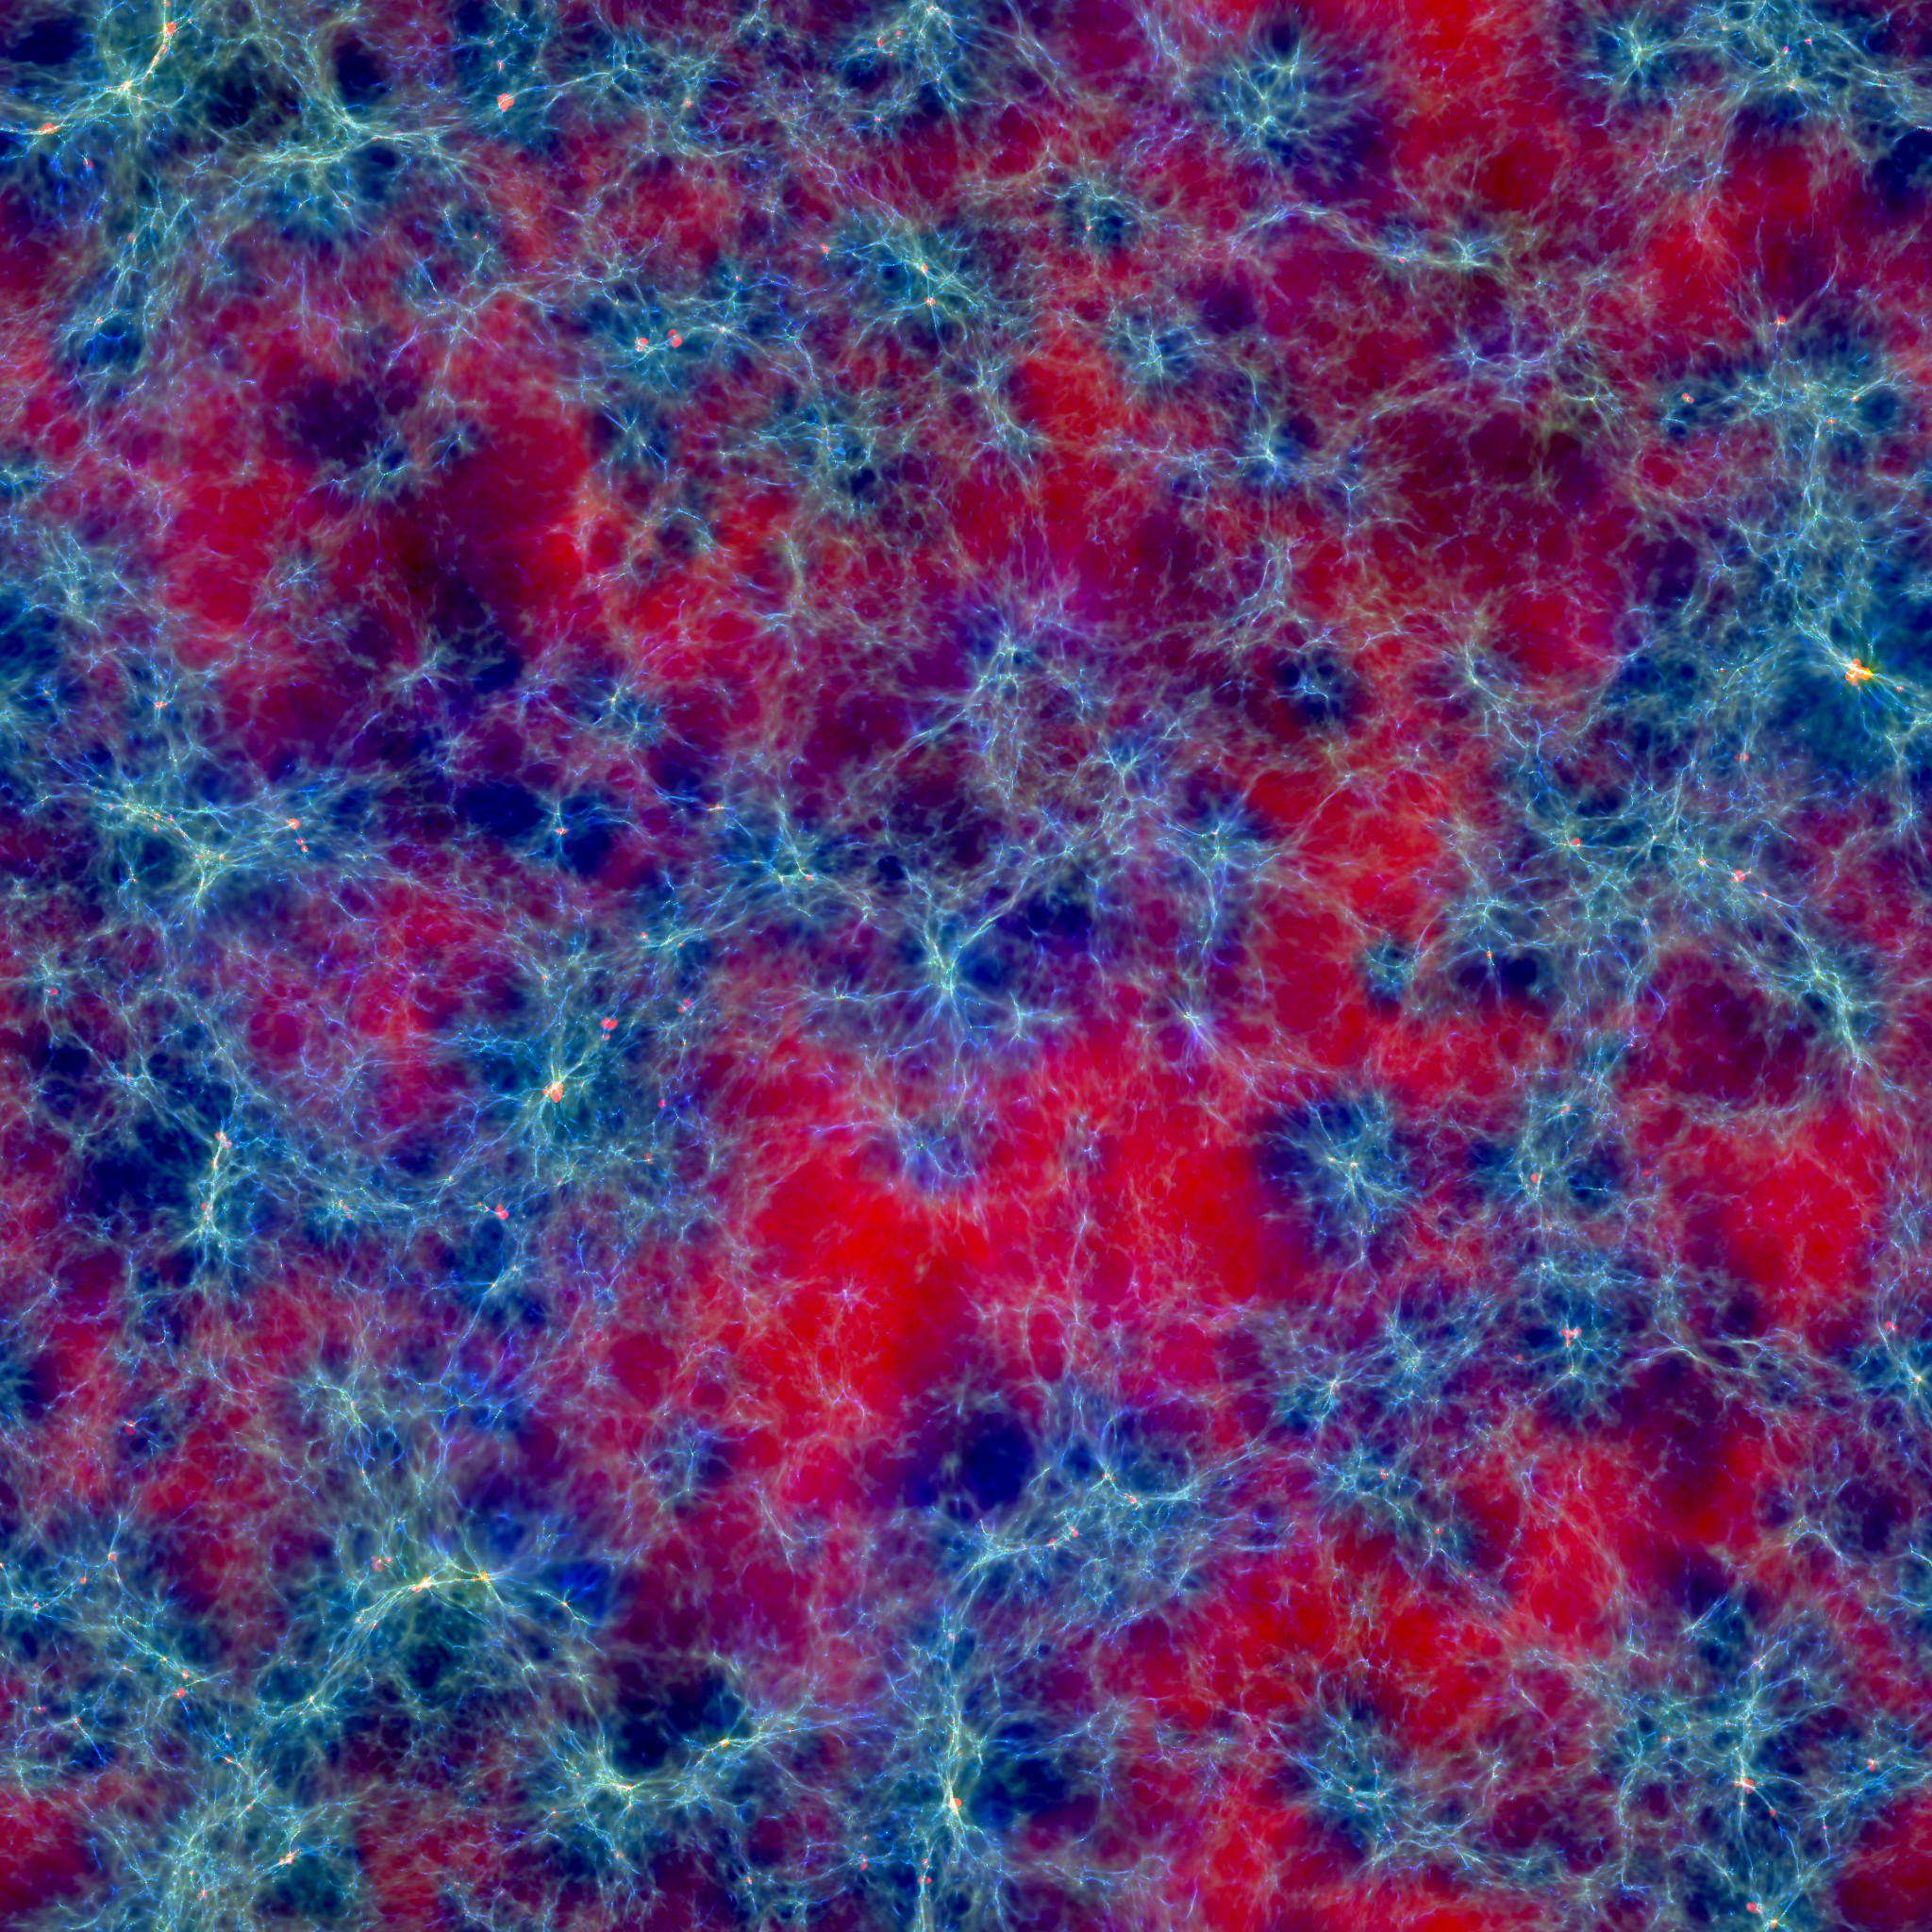
\includegraphics[width=.95\linewidth]{img/04/rgb-compose.jpeg} 
        \caption{Projection orthogonale de la simulation CODAII- EMMA en 2048$^2$.
        projection moyenne sur rho, T et rhoX en composition RGB.
Les zones rouges sont les vides qui ont recut du rayonnement plus tard et n'ont pas encore eu le temps de refroidir par détente adiabatique.  
        }
 		\label{fig:ortho}
\end{figure}

\section{Projection en perspective}
%opengl
%blender

Dans ce cas, il n'existe plus de façon directe de recuperer les lignes de visée, il est nécessaire d'avoir recours au lancé de rayon.
Cette technique appelée raycasting permet de récupérer toute les cellules interceptée pas un rayon donné.
Il existe différentes techniques de raycasting, j'ai pu en explorer plusieurs:

\subsection{L'algorithme de bressenham}
L'algorithme de bressenham est une technique optimisée de raycasting.
Il consiste a travailler sur l'indice des cellules d'une grille regulière.

Cette technique est tres rapide mais ne fonctionne cependant que sur grille regulière.

\begin{figure}[bth]
        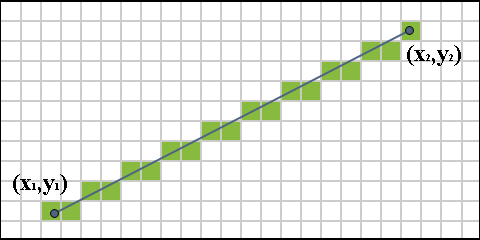
\includegraphics[width=.95\linewidth]{img/04/Bresenham_line.png} 
        \caption{Algorithme de Bressenham }
 		\label{fig:bressenham}
\end{figure}




\subsection{La méthodes KD-tree}

Une autre technique mise en place dans le but d'explorer directement l'amr.
De la mème manière que la technique de calcule des flux (TODO ref) cette technique repose sur l'utilisation d'un arbre pour determiner le cellule par lesquelles passent le rayon.





la mise en place de la camera
la définition de la position et du champs de vue (FOV) et de la profondeur de vue.
camera sphérique avec HealPix see Sec. \ref{sec:healpix}

la projection equirectangle est la projection la plus utilisée en photographie et video sphérique.
Elle présente un ratio d'aspect de 2:1 correspondant a 360:180.
L'association Healpix vers equirectangle est trivial puisque qu'elle consiste a associer les position x,y de la projection equirectangle, au angle $\theta$ et $\phi$ de la projection Healpix.
\begin{equation}
x=\theta
y=\phi
\end{equation}

La densité de point n'etant pas uniforme dans ce reférentiel, il est necessaire de realiser une interpolation sur une matrice régulière pour obtenir l'image finale. see Fig \ref{fig:equirectangle}


\begin{figure}[bth]
        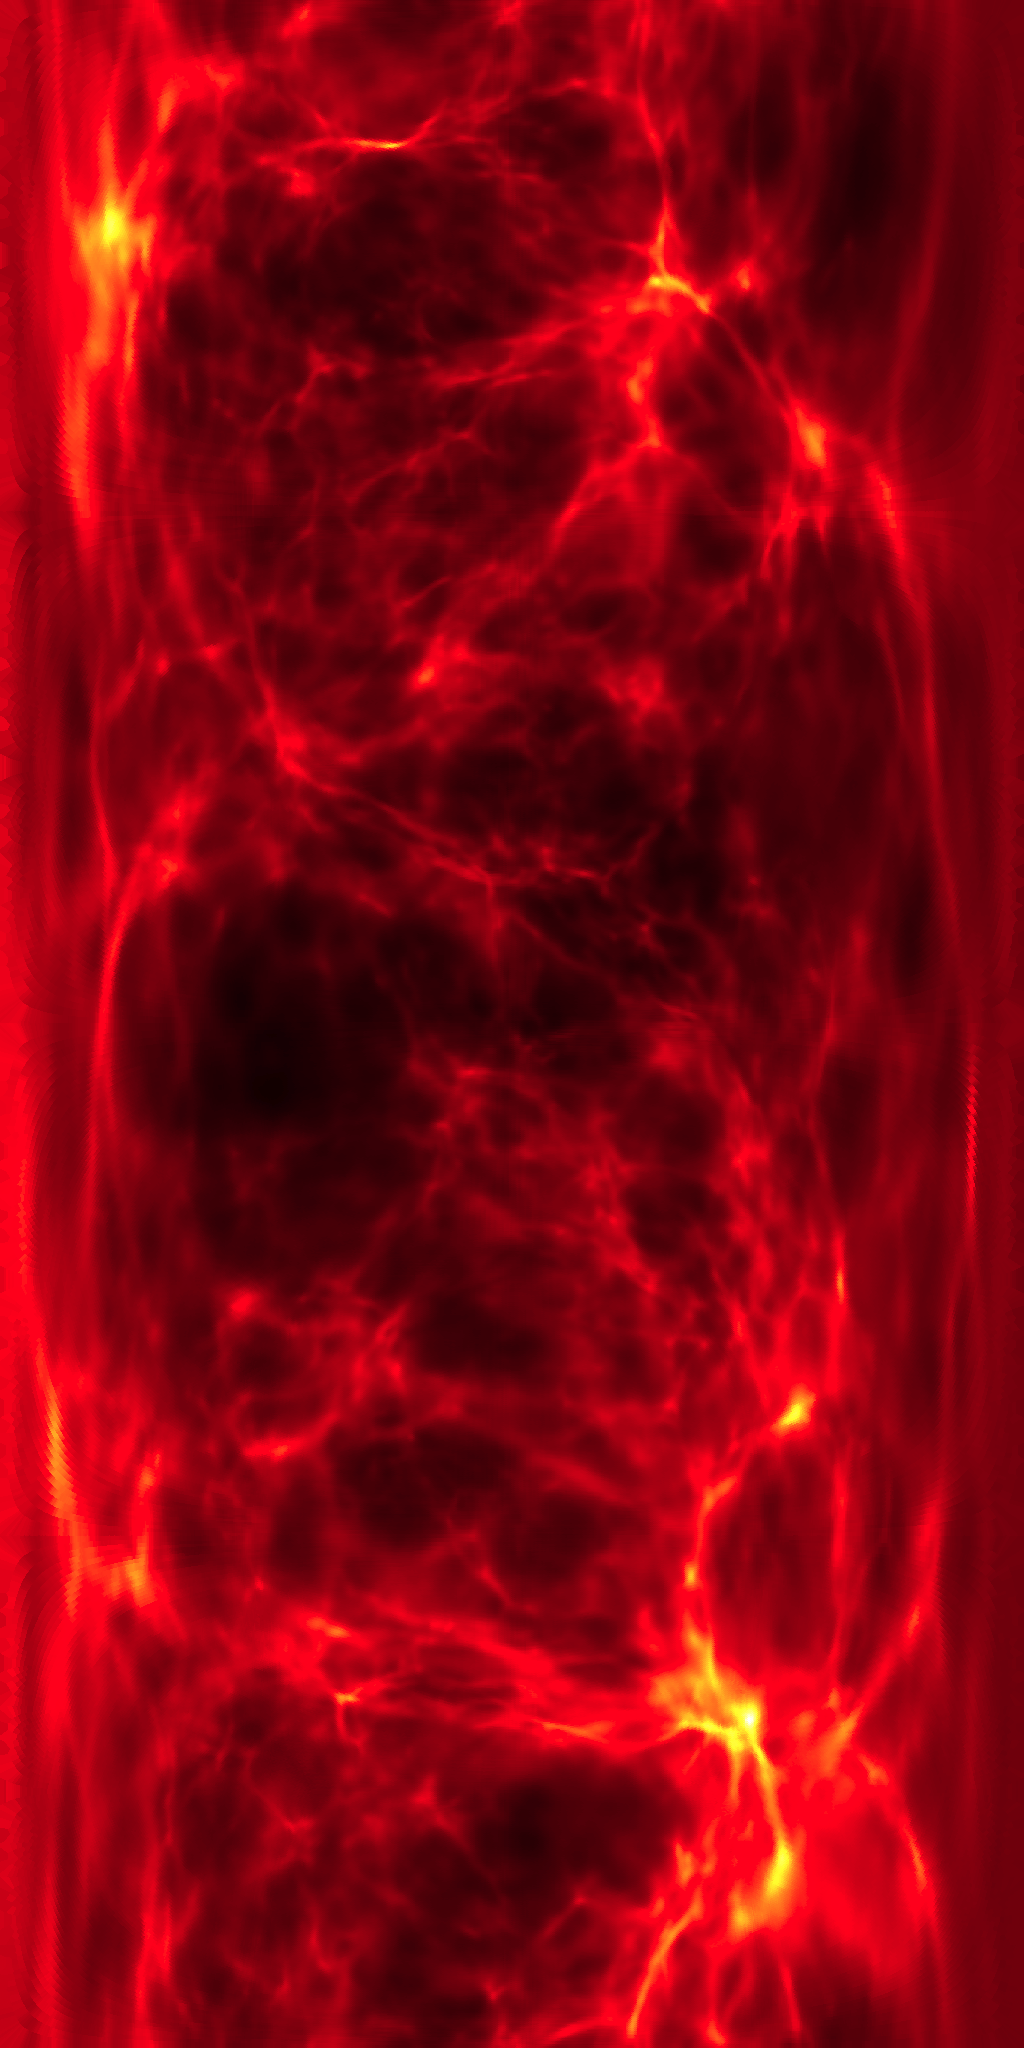
\includegraphics[height=.95\textheight]{img/04/equi.png} 
        \caption{Projection equirectangle d'une cube de densité.
        Ce type d'image représente une vue de 360° par 180° (d'ou un ration d'aspec de 2:1) ici prise depuis le centre de la simulation.}
 		\label{fig:equirectangle}
\end{figure}

Ce type d'image se prettent bien a la vulgarisation, car le resultat final est légé et peut être utilisé avec un Google Cardboard par exemple pour obtenir une visualisation intéractive facilement rependable.

\section{le compositing RGB (A)}
Une fois les projections realisées il est possibles de les combiner en créant des images en fausses couleurs.

De maniere naturelle, J'ai utilisé le rouge pour  la température et la transparence pour l'ionization.
il reste le bleu et le vert.
Dans une première série d'images j'ai utilisé le vert pour la densité de gas et le bleu pour la densité de matière noire.

\subsection{le théorie des couleurs}
Comment créer du noir et blanc?


par la moyenne :
\begin{equation}
gray= (R+G+B)/3
\end{equation}

R,G,B=gray


par une ponderation spéciale correspondant a la capacité de l'oeil a voir certaine couleur, conservation de la luminance:
\begin{equation}
gray = R*0.2989 + G*0.5870 +B*0.1140
\end{equation}

R,G,B=gray




\section{Movie}
%implementation du mode movie de EMMA
%c'est la même chose que précedemment mais a chaque pas de temps, il faut l'implementer en live (en c) pour ne pas avoir a sortir toute les info.


J'ai implémenté dans EMMA, la possibilité d'obtenir une matrice 2D par pas de temps, représentant la projection orthogonale suivant un axe donné.
La projection est réalisée de la même manière que précédemment mais a la volée et a chaque pas de temps.
Le choix a été fait de réaliser la projection a la fin de chaque pas de temps coarse.
La résolution temporelle est donc la résolution temporelle du pas de temps coarse.
Comme la résolution temporelle des niveaux raffinés est plus importante que le niveau coarse, 
LA projection temporelle peux etre 
En écrivant ces lignes je me rends compte que le dt de projection devrait être lié au dx de projection. 

Les simulations que j'ai pu réalisées comportaient environs un millier de pas temps, et généraient donc autant d'images ($N_{dt} \approx 10^3$).
A 25 FPS cela représente une durée de 40 secondes de vidéo.




\section{Light cone}
La création d'un light cone se fait a partir des images générer par le mode movie.
Le cube est 

Si les images en sorties du mode movie on une résolution $N_p=1024$ pixel carré.
On prend une tranche d'une épaisseur $dx$ donnée suivant l'axe $y$ sur l'image du pas de temps $i_{dt}$, puis une deuxième tranche de la même épaisseur, mais décalée dans l 'image $i_{dt+1}$, et ainsi de suite.

La position du début $S_i$ et de la fin $S_f$ de la tranche dans l'image sera :

\begin{equation}
S_i = (dx * i_{dt}) \% N_p 
\end{equation} 
\begin{equation}
S_f = S_i + dx 
\end{equation} 

Le modulo sur la taille de l'image permet de gérer les conditions périodiques simplement.
On prendra également garde a utiliser une épaisseur de tranche qui soit un multiple entier du nombre de pixel de l'image de manière a respécter simplement les condition périodique

Le ratio d'aspect $\Phi$ est le rapport entre la hauteur et la longueur de l'image, et s'exprime :
\begin{equation}
\Phi = \frac{ N_{dt} * dx}{N_p}
\end{equation}
Étant donné que $N_{dt}$ et $N_p$ sont fixés par les paramètres de la simulation, il n'est possible de géré le ratio d'aspect qu'en fonction de l'épaisseur de la tranche $dx$, 

Plus le ratio d'aspect sera important, plus les structure vont se répétée sur le light cone.

Un light cone réaliser avec cette méthode et a partir d'une simulation présenté dans la partie %TODO ref
est présenté sur la figure \ref{fig:lightcone}


\begin{figure}[bth]
        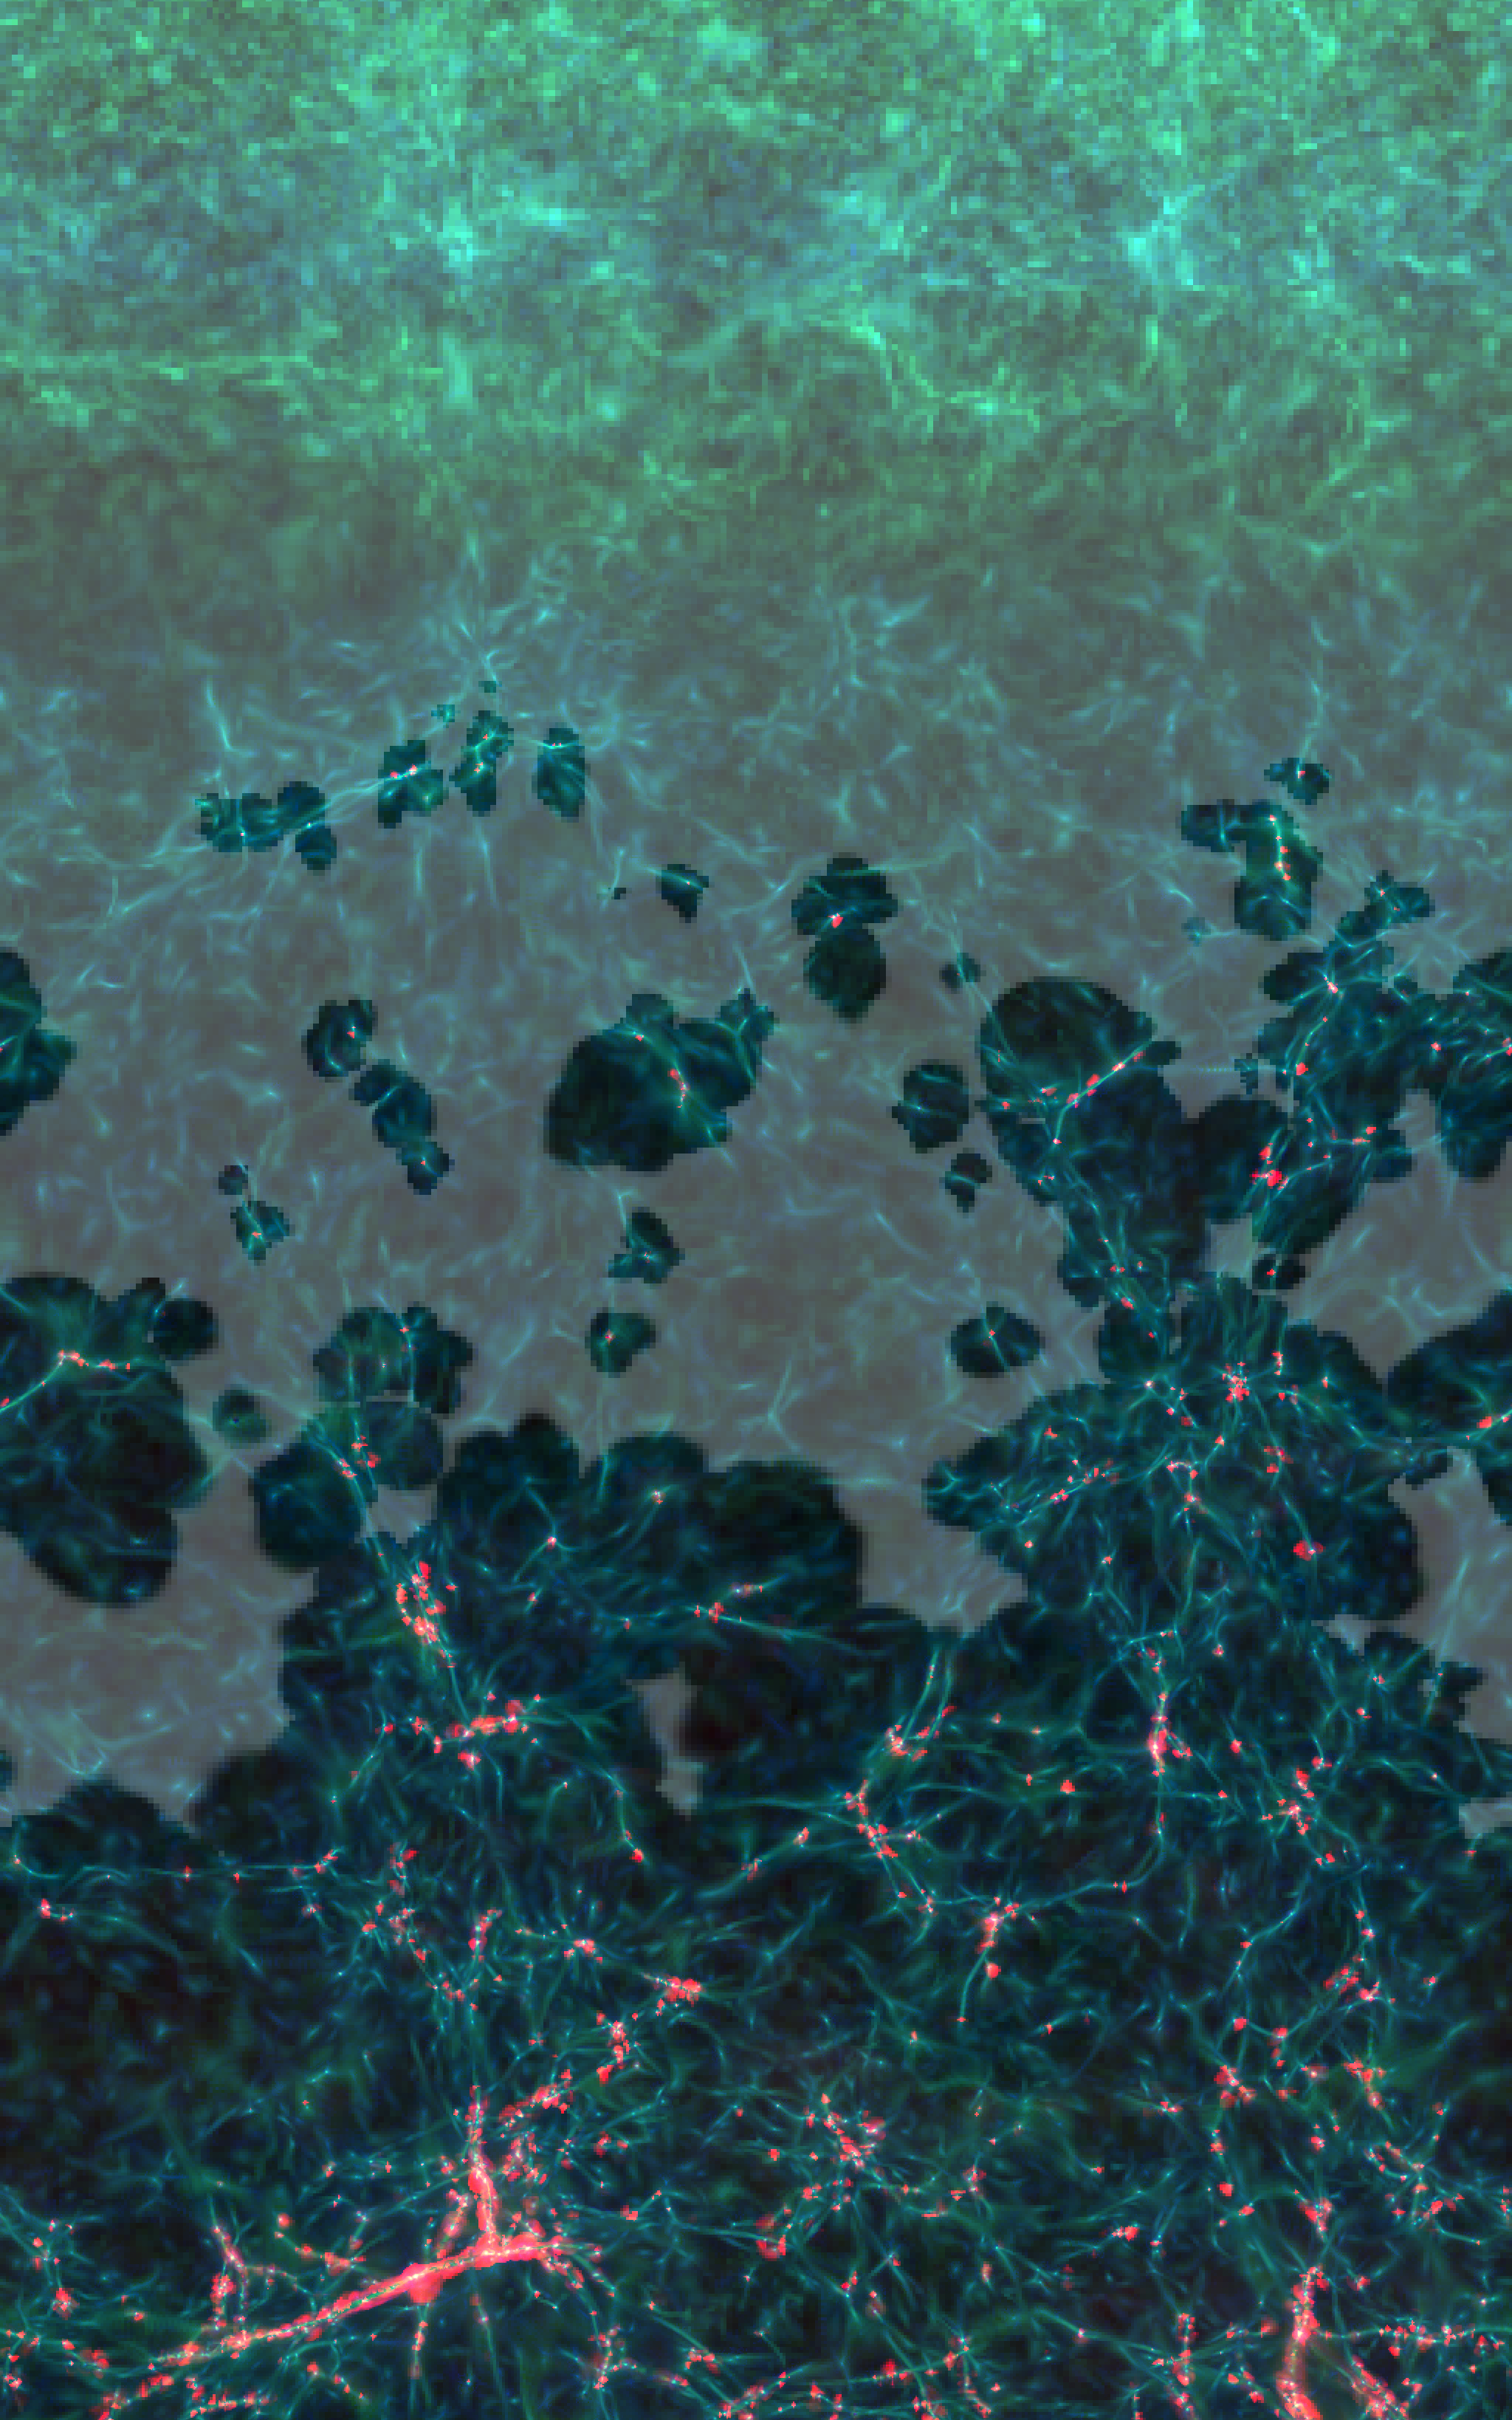
\includegraphics[height=.95\textheight]{img/04/frise_wall.png} 
        \caption{Light cone dans une simulation $8/h Mpc ^3$. Le temps se déroule de haute en bas sur plus de 700 Myrs }
 		\label{fig:lightcone}
\end{figure}

\section{Projeter des particules en 3D}

\subsection{avec un frame work} 

Blender 
interface python
Logiciel de visualisation 3d
Possibilité de faire du rendu volumique de qualité professionnelle
Pas adapté a la visu scientifique.


Irlicht
Moteur de jeu 3d open source 
extremement simple d'utilisation
les particules sont des bilboard : de texture 2d qui pointent tjrs vers la caméra
posibilité de customiser les points
deplacement en temps réel dans l'univers 3D a la manière d'un FPS
(tres) mauvaise performance 



\subsection{Sans Framework}

J'ai develloper un visualisateur de particule en OPenGL

Une capture d'écran du rendu de ce viewer est présenté sur la figure \ref{fig:viewer}

LEs partivule sont des vertex en language OpenGL.

declaration de buffer, envois sur la carte graphique.


Prochain objectif, ajouter du mouvement.

Interpolation entre 2 snaps.

interpolation faite en CUDA pour éviter les retour de GPU vers CPU.

posibilité d'utiliser plusieurs snaps 

Visualisation de la formation des structure en temps réélle tres instructive



\begin{figure}[bth]
        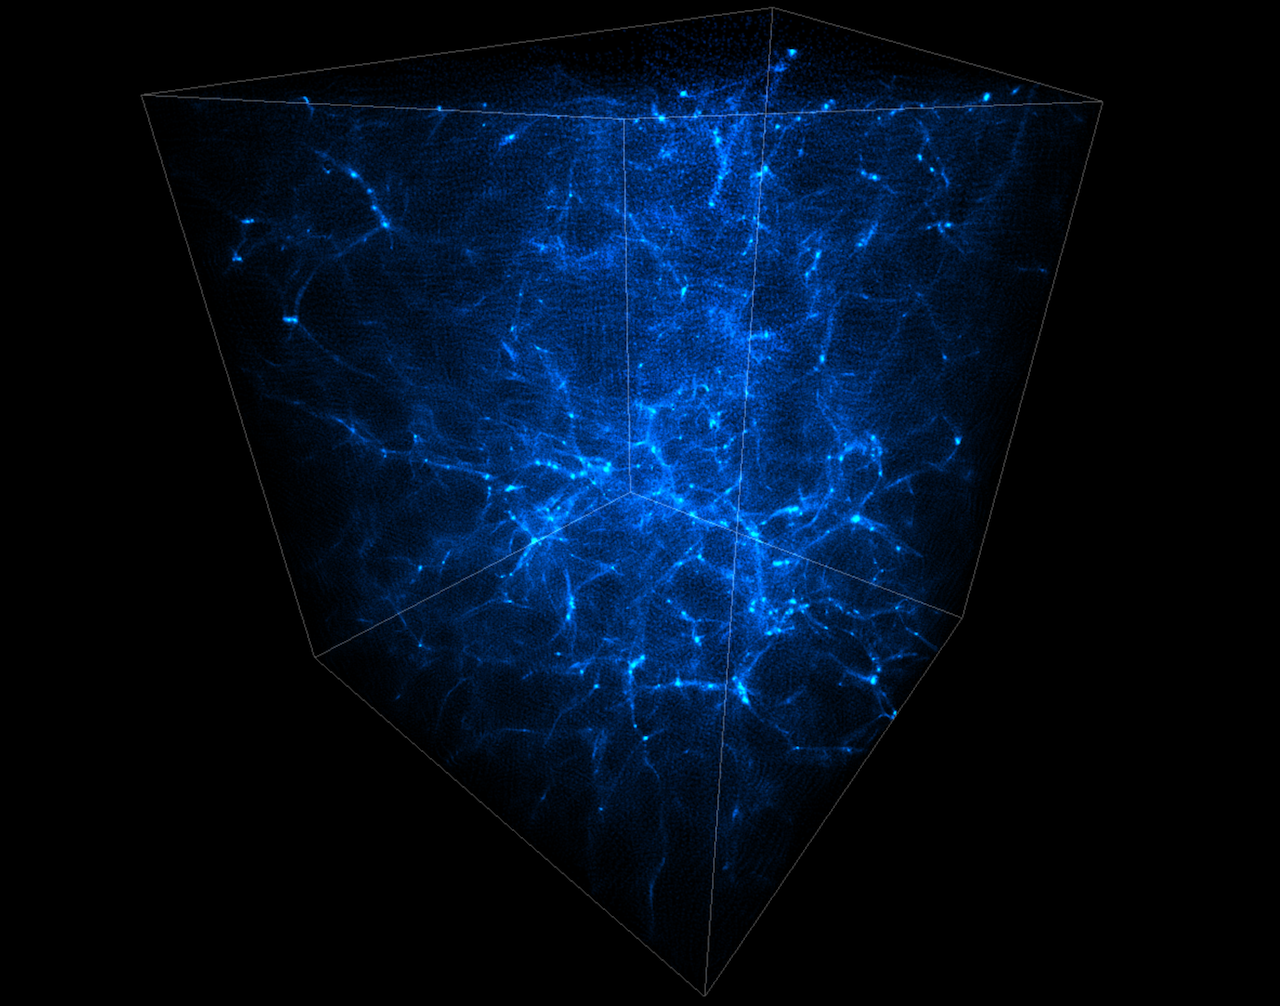
\includegraphics[width=.95\linewidth]{img/04/part.png} 
        \caption{Capture d'ecrandu viewer 3D  }
 		\label{fig:viewer}
\end{figure}